\documentclass[../main.tex]{subfiles}
\begin{document}
\section{Alcance del Proyecto}
\begin{enumerate}

\item Lo que logré realizar:
	\begin{itemize}
	\item Cargar documentos XML bien estructurados, que no contengan la línea de declaración y donde cada línea es:
	\begin{enumerate}
		\item Sólo una etiqueta de cierre.
		\item Sólo una etiqueta de apertura.
		\item Sólo una etiqueta de cerrado automático.
		\item Sólo un fragmento(o todo) del contenido de una etiqueta.
	\end{enumerate}
	Ejemplo:
	\lstset{language=XML}
		\begin{lstlisting}[caption= Documento que la aplicación si logra cargar, frame=none]
<tag1>
	<tag11 k1="a" k2="b">
		<sct t1="x" t2="y"/>
		tag11Content
	</tag11>
	<tag12 k1="c" k2="d">
		tag12Content
	</tag12>
	<tag12 k1="e" k2="f">
		tag13Content
	</tag12>
	Tag1Content
<tag1>
		\end{lstlisting}
	\clearpage
	\item Cada nodo XML es en sí un objeto de la clase xml, cuyo método constructor se muestra en el cuadro:
		\lstset{language=Python}
		\begin{lstlisting}[caption= Método constructor de la clase xml, frame=none]
	def __init__(self, tagName, parent = 'noParent', attributes = 'noAttributes', children = 'noChildren', content = 'noContent'):
		self.__parent = parent #Objeto de la clase string.
		self.__tagName = tagName #Objeto de la clase string.
		self.__attributes = attributes #Objeto de la clase dict.
		self.__children = children #Lista de objetos de la clase XML.
		self.__content = content #Objeto de la clase string.
		\end{lstlisting}
	
	\begin{figure}[!ht]
		\begin{center}
                		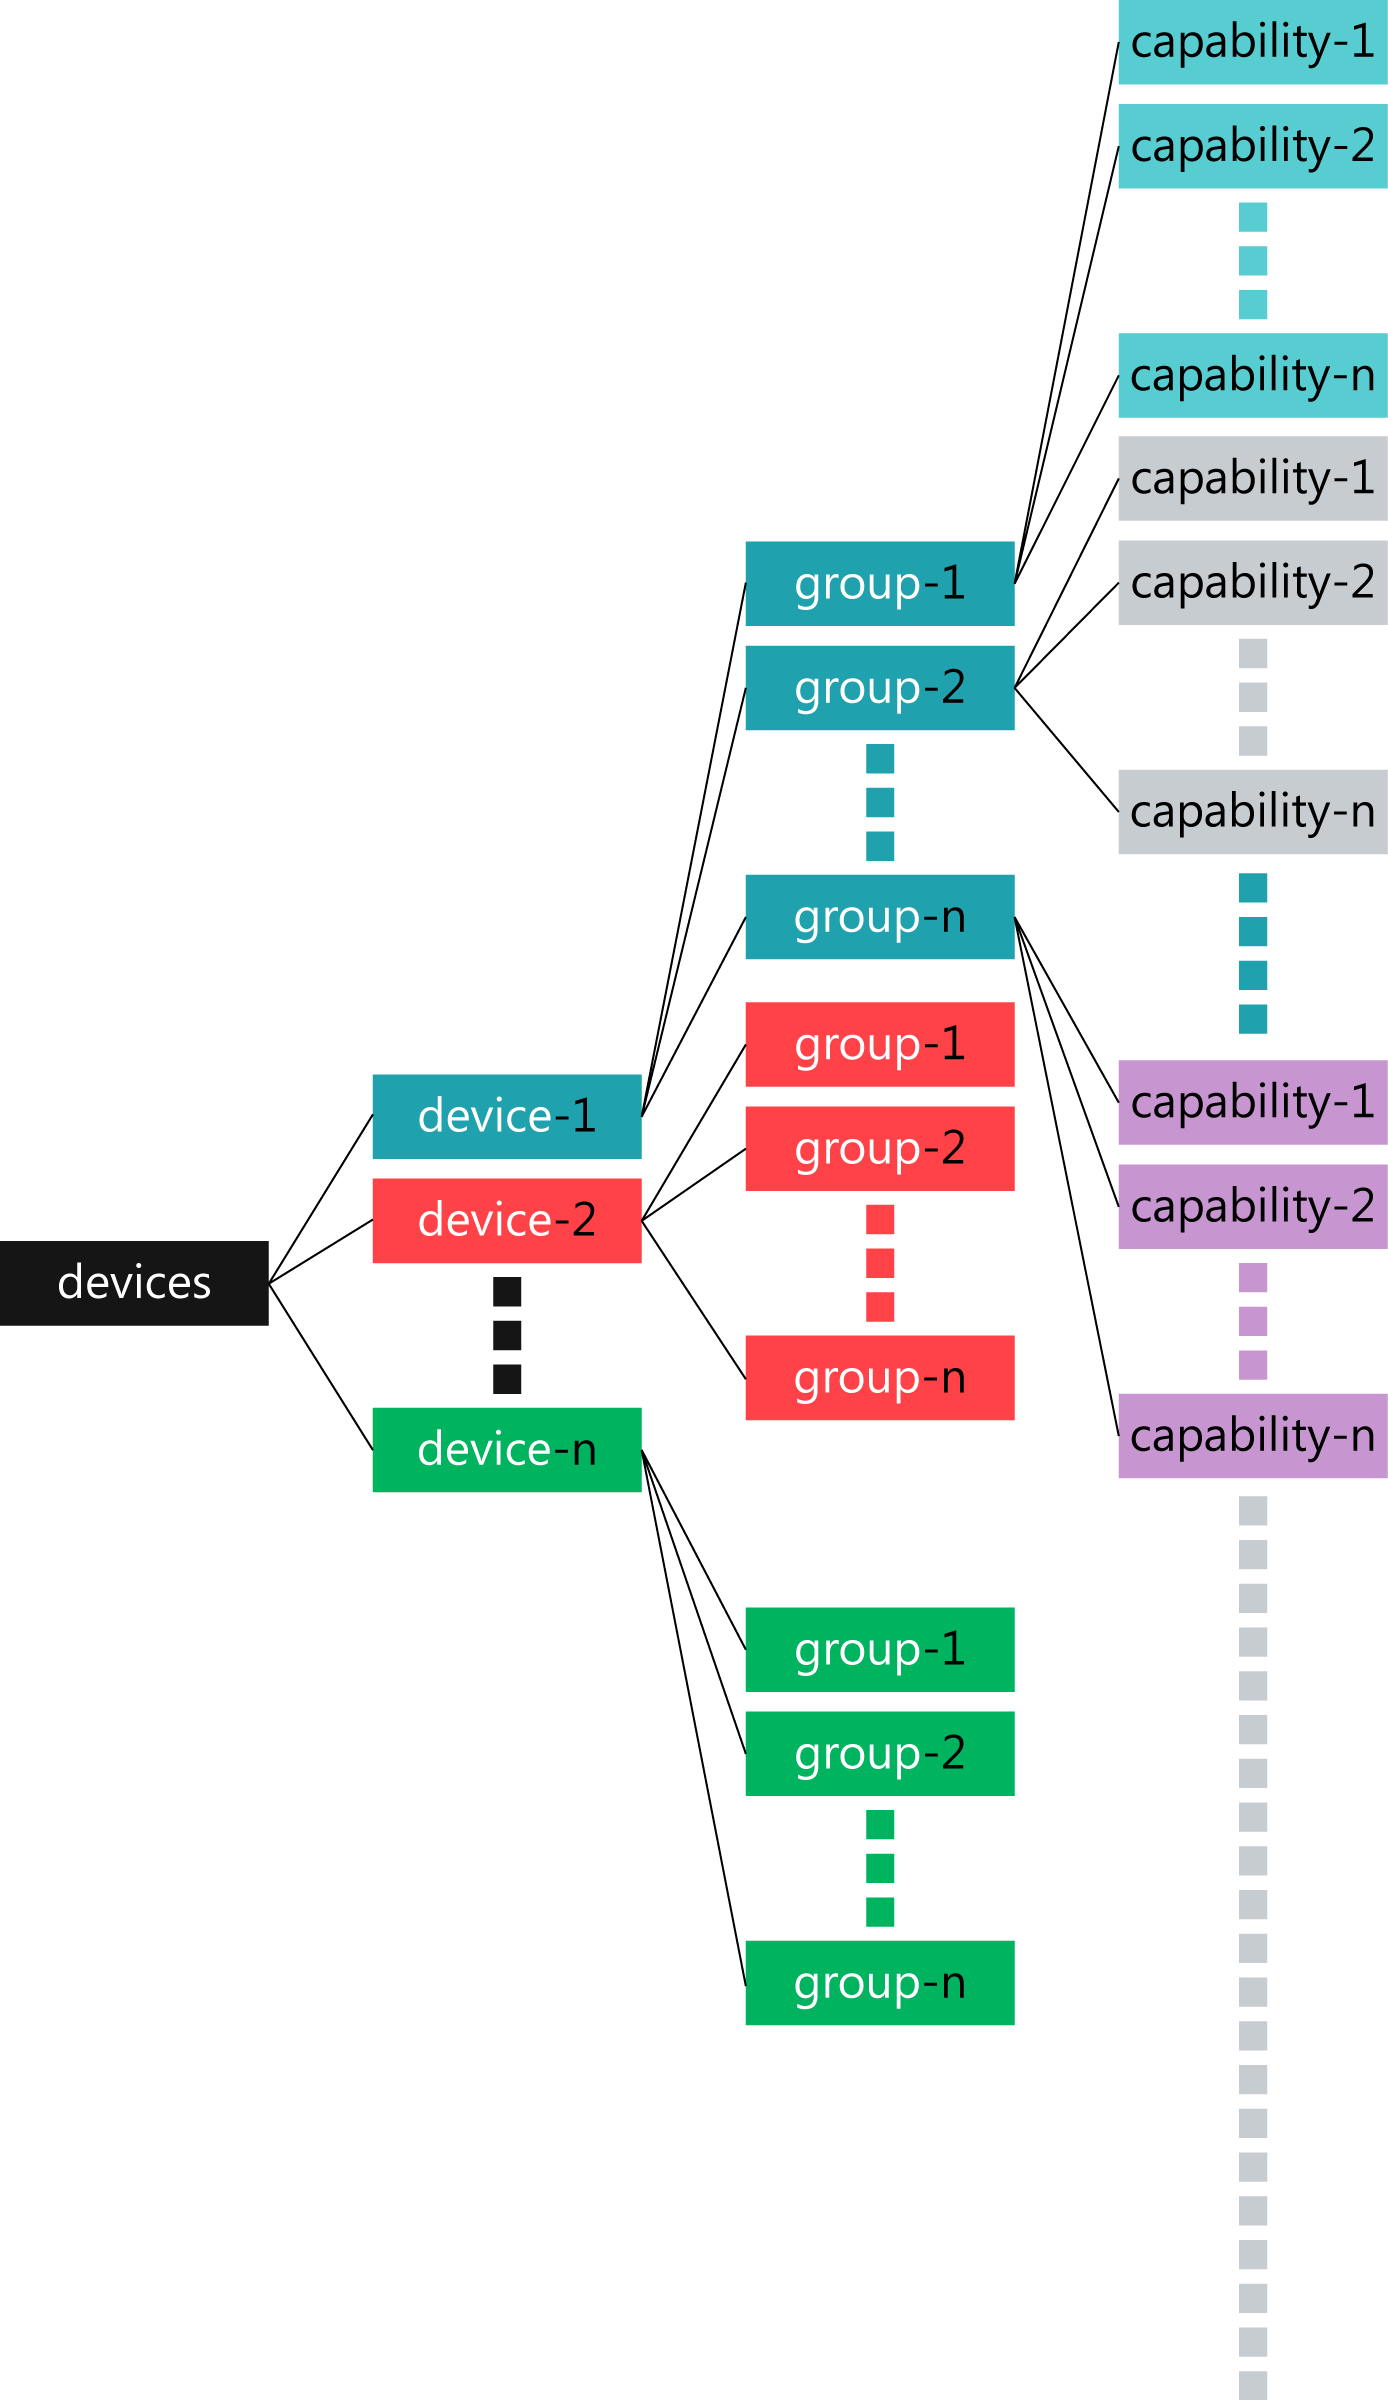
\includegraphics[width=0.8\textwidth]{./images/tree.png}
        		\end{center}
        		\caption{Árbol XML}
        	\end{figure}
        	 \item Cargar un fragmento del documento wurfl-2.3. Específicamente la aplicación logra cargar en memoria el árbol  mostrado en la Figura 2.1.
	 \item Realizar diferentes tipos de búsquedas en la estructura creada. Hasta ahora he implementado 3 funciones para realizar búsquedas:
	 	\begin{enumerate}
	 		\item getDBID, la cual que recibe como parámetros el nombre del dispositivo y una referencia al nodo raíz y retorna una referencia al dispositivo que posee el nombre pasado como parámetro, caso contrario retorna None.
	 		\item getCapabilityValue, la cual me permite obtener el valor de una capacidad determinada si se conocen el nombre de la capacidad y el nombre del dispositivo (o una referencia al dispositivo)
	 		\item getDevicesWithCapVal, que permite recuperar todos los dispositivos que poseen en común un valor determinado para una capacidad determinada, si se conoce el nombre de la capacidad, una referencia al nodo raíz, y opcionalmente el valor de la capacidad.
	 	\end{enumerate}
	 \end{itemize}
	 
	 \clearpage
 \item Lo que no logré realizar:
 	\begin{itemize}
 	\item Determinar si un documento XML está bien estructurado.
 	\item Cargar documentos XML en donde exista una línea (o más) que posea una etiqueta de apertura y cierre en si misma. Ejemplo:
 	\lstset{language=XML}
		\begin{lstlisting}[caption= Documento que la aplicación no logra cargar, frame=none]
<tag1>
	<tag11 k1="a" k2="b">
		<sct t1="x" t2="y"/>
		tag11Content
	</tag11>
	<tag12 k1="c" k2="d">tag12Content</tag12>
	<tag12 k1="e" k2="f">tag13Content</tag12>
	Tag1Content
<tag1>
		\end{lstlisting}
 	\end{itemize}
\end{enumerate}
 \end{document}